\chapter{脉搏波特征点检测及特征参数集的构建}
\section{引言}
前文已经阐述过,光电容积脉搏波(PPG)本身蕴含着丰富的血液动力学信息,其形态、强度、速率、节律等特征反映心脏的功能与状态,也可以反映出各级动脉及分支中血管壁弹性、血管阻力、血液黏度等信息。但同时,PPG信号也与其他医学电生理信号类似,
易收到多种噪声干扰。本章着重解决脉搏波信号的预处理问题与脉搏波描述等两个问题。前者主要涉及信号处理过程,后者则是寻找、挖掘、设计数字特征对量化描述脉搏波。最后,本章将多种脉搏波量化特征进行了汇总,构建了脉搏波一般描述特征集合。
本章对以上过程中涉及的概念及算法分别给出了原理及设计思路说明,而其中关于软件流程的功能性设计可参阅本论文第六章节相关内容。
\section{信号预处理}
本小节着重解决如何提高原始信号质量并正确定位PPG相关特征点、检测完整脉搏波波形等内容。\autoref{fig:samplesignal}展示了一段有代表性的经由GE B650监护仪实际采集的PPG信号,从中可以看到所得信号整体信号质量较高,但仍然有基线偏移、
PPG信号重博波特征不明显等问题。这些问题可能与具体硬件检测电路、使用传感器种类及监护仪处理算法有关。此外,可以看到\autoref{fig:samplesignal}仍然有一段明显的无效数据段(约40s-55s期间内),在实际处理时需要对其进行剔除。
由于重博波特征不明显无法经由软件算法人工恢复,故本章节暂不对任何重博、切迹进行计算处理,后续也无任何与之相关的PPG信号特征参数。本章涉及的信号分析流程如\autoref{fig:process}所示。
\begin{figure}[htbp]
    \centering
    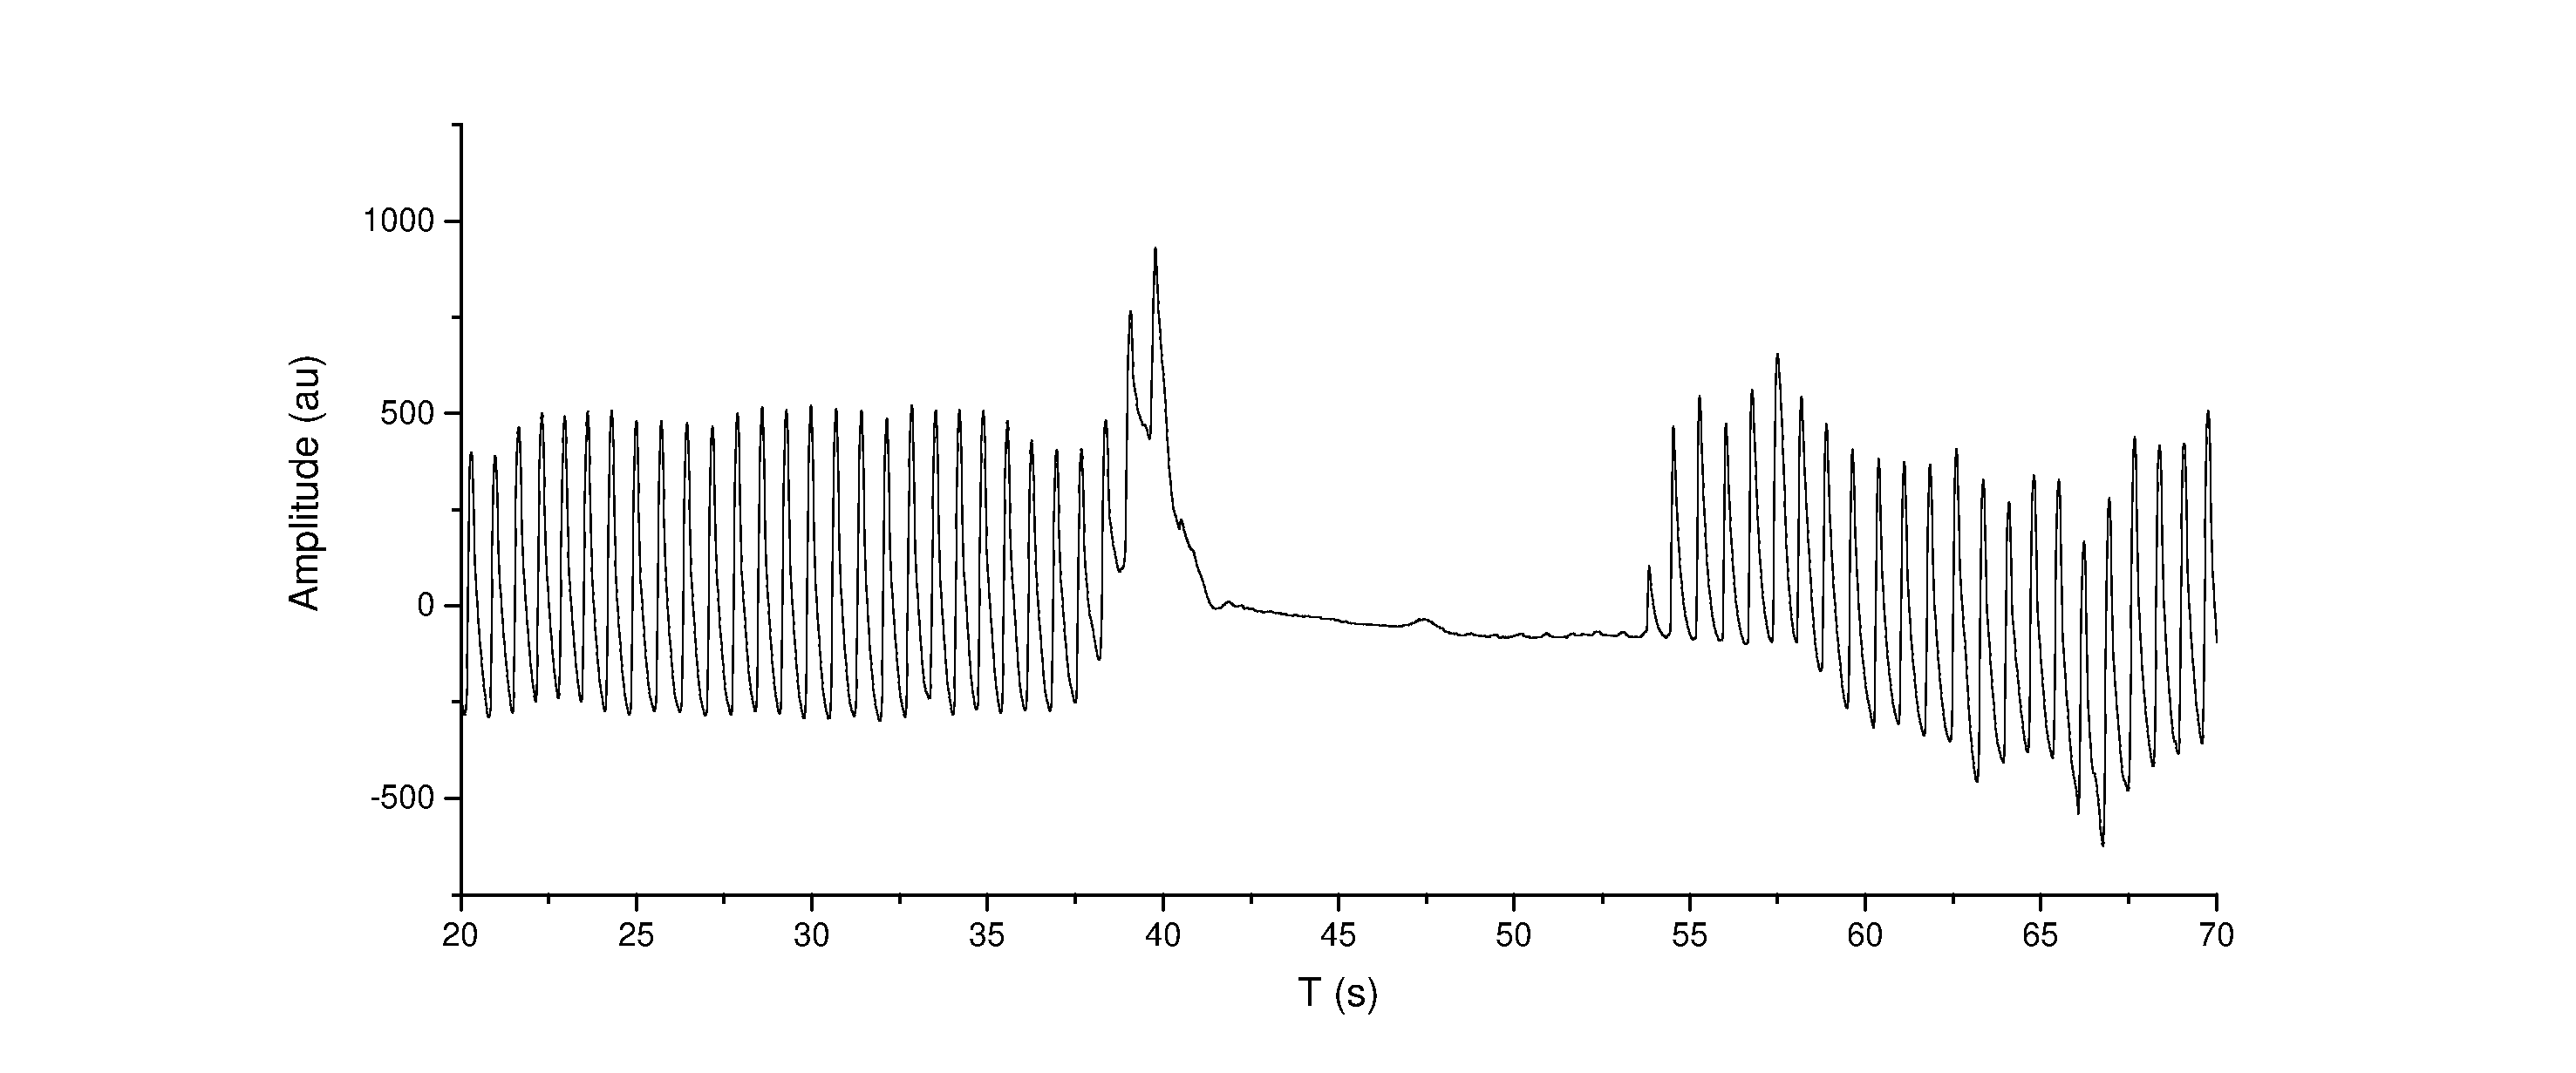
\includegraphics[width=0.9\linewidth]{ch4/sampleSignal}
    \caption{\label{fig:samplesignal}一名被试实采PPG信号(片段)}
\end{figure}
\begin{figure}[htbp]
    \centering
    
\includegraphics[width=\linewidth]{ch4/process.pdf}
    \caption{\label{fig:process}信号预处理流程示意}
\end{figure}

\subsection{信号滤波}

\subsection{波形检测}
脉搏波波形的正确检测是后续所有特征计算的基础,波形检测的准确性及抗干扰能力显得尤为重要。传统的波形检测一般都是对波形进行一次性检测,然后再人工判别检测的准确性。本小节则改进了这一流程,充分利用“宽进严出”的筛选原则,
利用PPG波峰的局部最大值原理进行初筛,随后,对按照多种标准对初筛结果进行复核确认,最终按照预设的策略有选择的得到最终波形检测结果,这一过程如\autoref{fig:detect}所示。
\begin{figure}[htbp]
    \centering
    
\includegraphics[width=\linewidth]{ch4/detect}
    \caption{\label{fig:detect}波形检测流程示意}
\end{figure}

一、波形检测

波峰与波谷是脉搏波的最基本特征点,也是检测波形其他特征点的基础。顾名思义,波峰是特定PPG波形内的最大值,在其左邻域内PPG幅值单调递增,右邻域内PPG幅值单调递减。

检测分别波峰,波谷 再按规则进行时间组装对应

2

二、异常信号处理

对正常PPG波形,上述检测算法可以实现较好的检测效果,但对干扰信号的检测能力不足,使得具有且仅具有PPG波形一般特征的“疑似波峰”得到确认并保留,

1.评估标准

\Rnum{1}.能量

\Rnum{2}.方差

\Rnum{3}.时间

\Rnum{4}.其他



2.决策过程

当上述多个PPG波形评估器构建完成后,对PPG初筛待检波形均会生成一定的输出——正确检测波形或错检干扰。该过程可抽象成使用多个学习器$h_i$从类别标记集合$\{c_0,c_1,\cdots,c_N\}$中产生最终输出。则此时可借鉴集成学习中的投票策略(voting)完成对初筛波形的最终判别
决策\cite{Zhou2016}。若将$h_i$在样本$x$上的预测输出表示为$N$维向量$(h_i^1(x);h_i^2(x);\cdots;h_i^N(x))$,则常见可用的投票策略包含以下三种\cite{Kittler1998,Zhou2016}:

\Rnum{1}.绝对多数投票法

若某标记得票数超过半数,则预测为该标记,否则拒绝该预测。
\begin{equation}
    \label{equ:mvoting}
    H(x)=
    \left \{
    \begin{aligned}
        c_j,&\quad if \sum_{i=1}^T{h_i^j(x)}>0.5\sum_{k=1}^N{\sum_{i=1}^T}{h_i^k(x)}\\
        reject,&\quad otherwise.
    \end{aligned}
    \right.
\end{equation}

\Rnum{2}.相对多数投票法

应用绝对多数投票法时,若对所有标记类别,其得票数均不超过半数,则此时无法得出投票结果。为避免此情况发生,相对多数投票法直接将预测为得票最多的标记。若同时有多个标记获得最高票,则从中随机选取一个作为最终结果。
\begin{equation}
    \label{equ:pvoting}
    H(x)=c_{arg \max\limits_{j} \sum_{i=1}^T{h_i^j(x)}}
\end{equation}

\Rnum{3}.加权投票法

与前面两种投票法不同,加权投票法给所有的学习器$h_i$以特定的权重$w_i$,将所有可能汇总后得到最后的标记类别,
\begin{equation}
    \label{equ:wvoting}
    H(x)=c_{arg \max\limits_{j} \sum_{i=1}^T{w_ih_i^j(x)}}
\end{equation}
其中,$w_i\ge0$,$\sum_{i=1}^T{w_i=1}$。

\autoref{equ:mvoting}至\autoref{equ:wvoting}并没有限制单个学习器输出值类型,而常见的学习器输出值$h_i^j(x)$有类标记与类概率两大类。而基于这两类输出值进行的投票也相应被称为硬投票与软投票,类标记与类概率的特点可总结概括为\autoref{tab:vote}所示。
需要注意的是,硬投票可能会导致最终的分类结果由多数概率值较低的学习器决定,而非概率更高、更有分类把握的少数学习器。因此,在条件允许的情况下,应尽可能使用软投票机制进行决策。
\begin{table}[htbp]
    \centering
    \caption{\label{tab:vote}类标记与类概率特点对比}
    \begin{tabularx}{\linewidth}{c|X<{\centering}X<{\centering}}
        \Xhline{1pt} 
            &\textbf{类标记}&\textbf{类概率}\\
        \hline
        \textbf{$h_i^j(x)$值域}  &$\{0,1\}$    &$[0,1]$     \\
        \textbf{$h_i^j(x)$输出说明}&\tabincell{c}{若$h_i$将样本$x$预测为$c_j$\\则取值为1,否则为0}&\tabincell{c}{$h_i^j(x)$相当于对后验概率\\$P(c_j|x)$的一个估计}\\
        \textbf{投票策略}&\tabincell{c}{绝对多数投票法、\\相对多数投票法}&加权投票法\\
        \textbf{别称}    &硬投票 &软投票 \\
        \Xhline{1pt}
    \end{tabularx}
\end{table}

由于本研究尚未对上述PPG波形评估器的类概率进行相关研究,因而选择将各评估器的输出暂时直接限定为类别标记输出为0或1,最终基于硬投票策略进行初筛波形的类型判别。

三、检测算法性能评估

1. 特定波形检测效果


2. 与标准标定数据库对比

\subsection{去除基线漂移}
在实际得到的PPG波形中,由于呼吸干扰等原因,一个完整PPG波形对应的两个波谷,即该波形的始末位置的幅值很难保持一致。这种差异最终会导致PPG信号的基线出现波动,也就是工程领域的基线漂移问题,如\autoref{fig:drift}所示。为满足后续特定PPG形态特征计算需求,
需要消除基线漂移的影响。此时一种基于线性变换的处理过程可以实现该目标。
\begin{figure}[htbp]
    \centering
    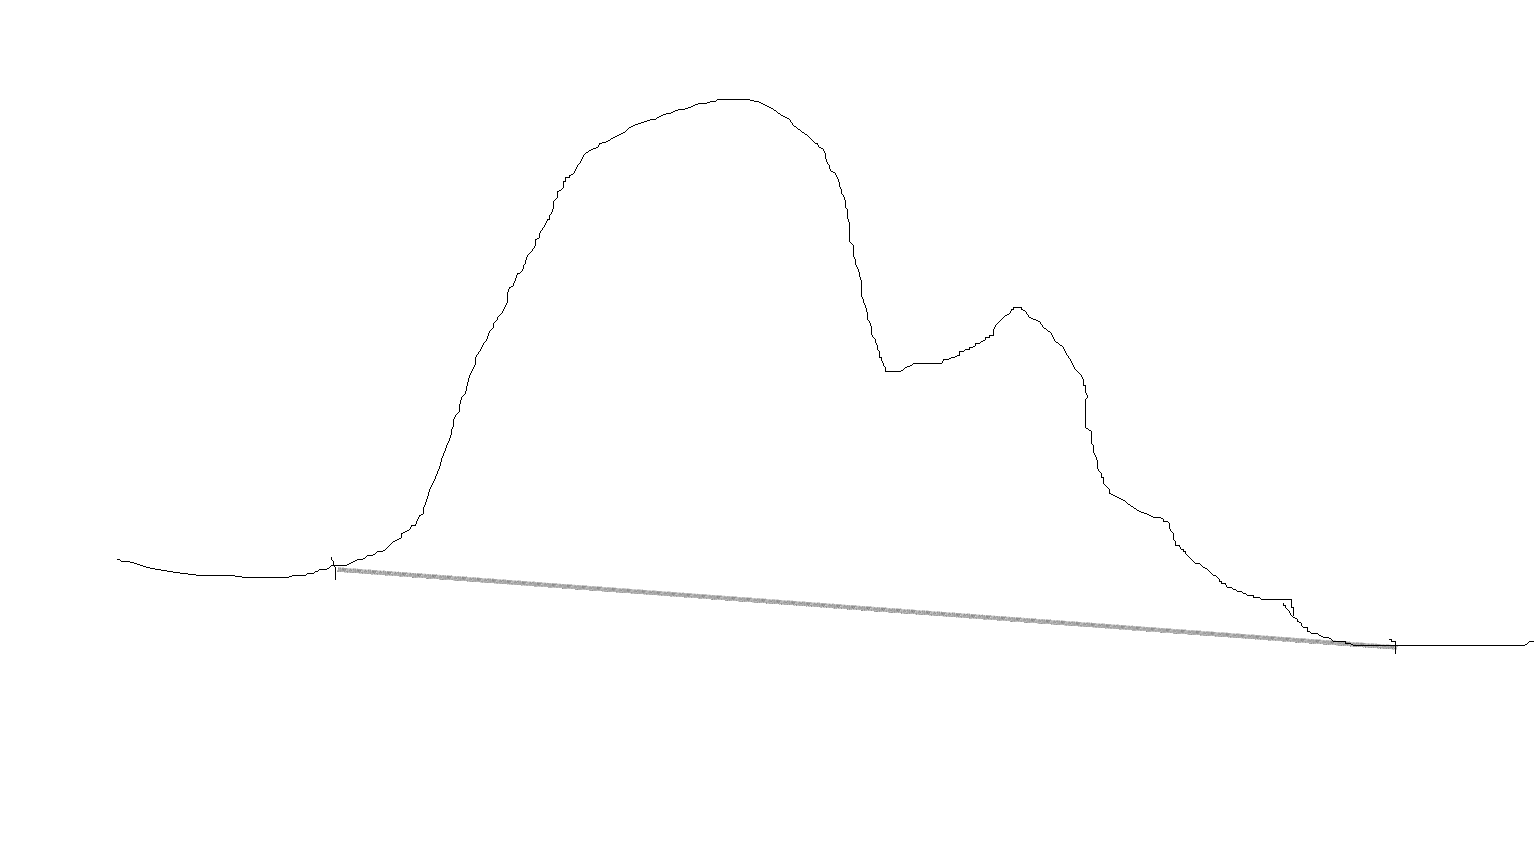
\includegraphics[width=.6\linewidth]{ch3/drift}
    \caption{\label{fig:drift}基线漂移去除示意及处理效果对比}
\end{figure}

如\autoref{fig:drift}所示,易知脉搏波的相对幅值$A$是采样时间$t$的函数,将其表示为$A(t)$。对任一特定波形,其起始点与终止点处对应的幅值可分别表示为$A(t_{start})$与$A(t_{end})$。
由于始末位置脉搏波幅值不等,则明显两者之间存在一条斜率不为0的直线,其具体值为
\begin{equation}
    \label{equ:linek}
    k=\frac{A(t_{start})-A(t_{end})}{t_{start}-t_{end}}
\end{equation}
则该直线上任意点即代表了在该时刻脉搏波波形与水平基线的偏移量,即
\begin{equation}
    \label{equ:liney}
    \Delta(t)=k(t-t_{start})+A(t_{start})
\end{equation}
此时,去除基线漂移后的脉搏波信号可标示为
\begin{equation}
    \label{equ:adjusta}
    A_{adjsut}(t)=A(t)-\Delta(t)
\end{equation}

\subsection{插值计算}
由于本章后部分自行定义设计的多种新型脉搏波特征,在特征计算过程中对脉搏波的采样频率有着较高要求。由于GE B450设备导出的原始脉搏波数据的采集频率仅为100$Hz$,难以满足后续计算。因此,需要在PPG预处理环节额外引入了插值计算操作以人工提高信号采样率。

插值是求值的逆过程,通过某些已知的数据点去推断一个(系列)特定的函数,使得所有已知数据点均在该函数图像上,从而去推断更多未知数据点,解决相应的实际问题,这一过程如\autoref{fig:spline}所示。
\begin{figure}[htbp]
    \centering
    \subfigure[经过点(1,2),(2,1),(4,4)和(5,3)的线性样条]{
    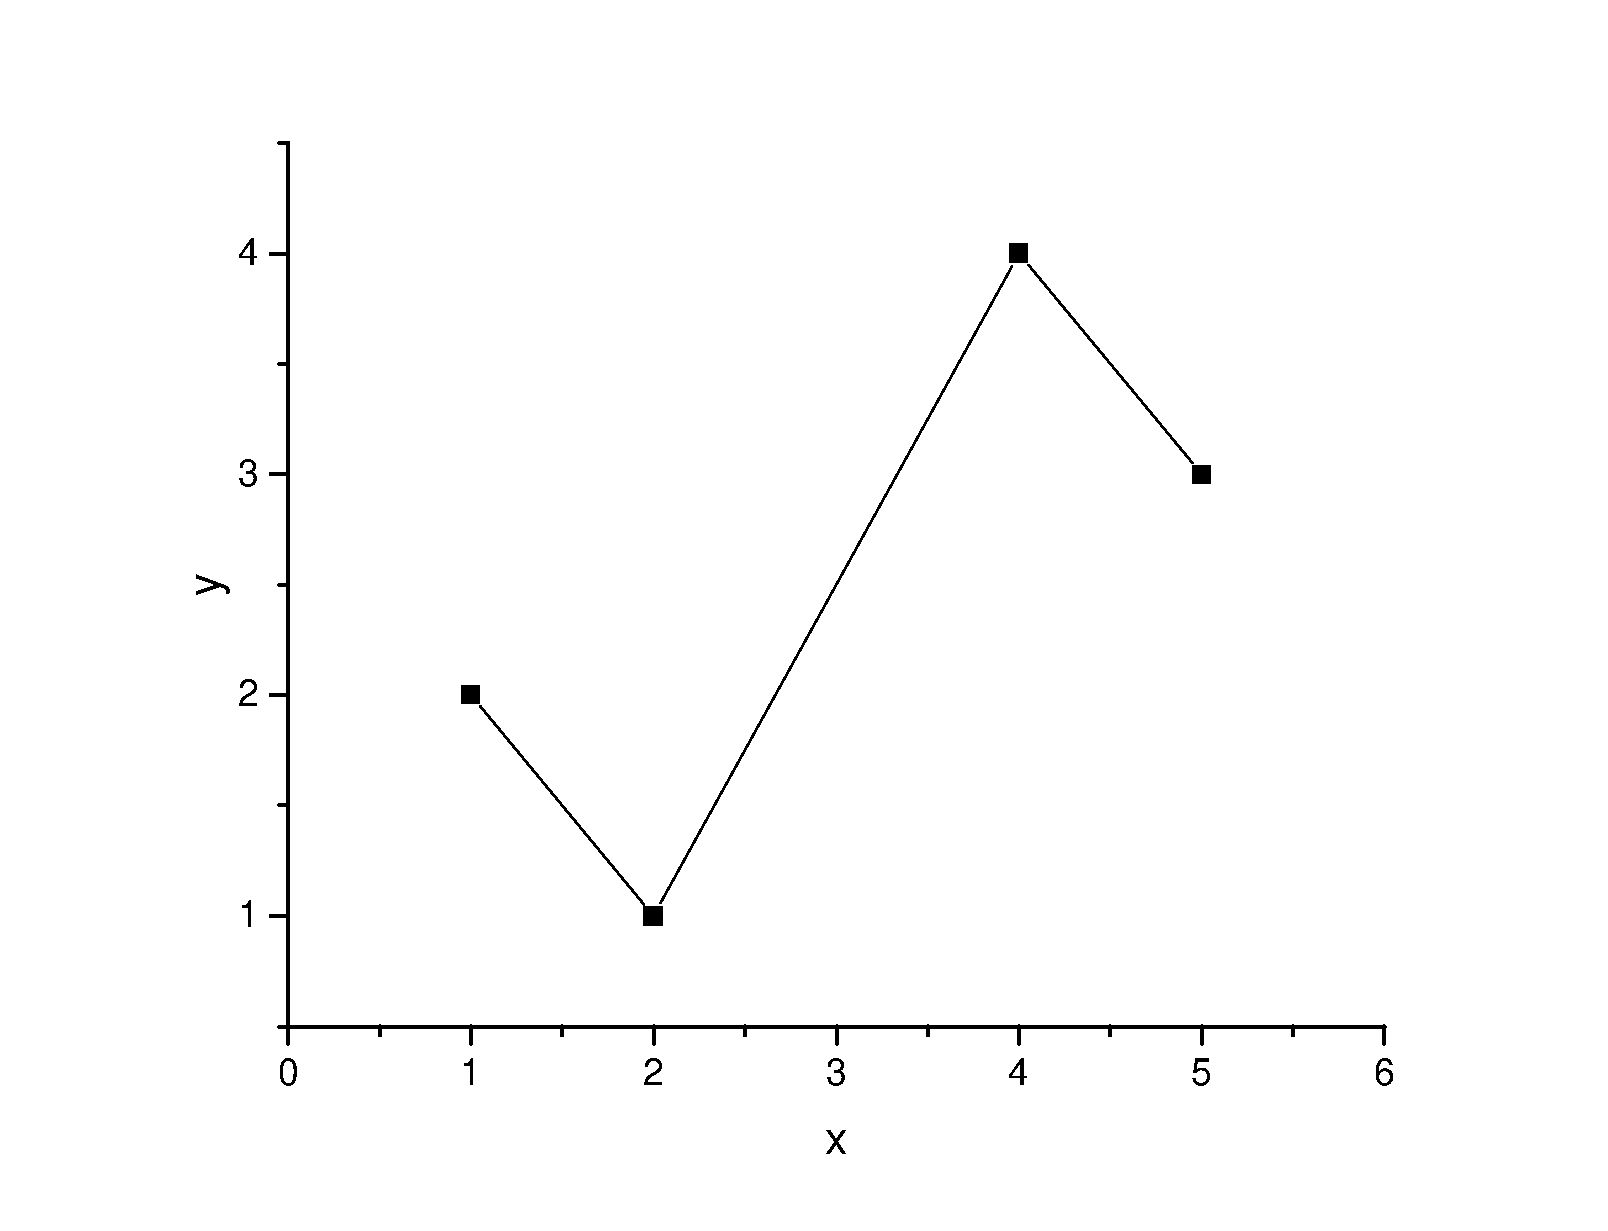
\includegraphics[width=5.5cm]{ch4/spline1}
    }
    \quad
    \subfigure[经过相同点的一种可能的三次样条插值]{
    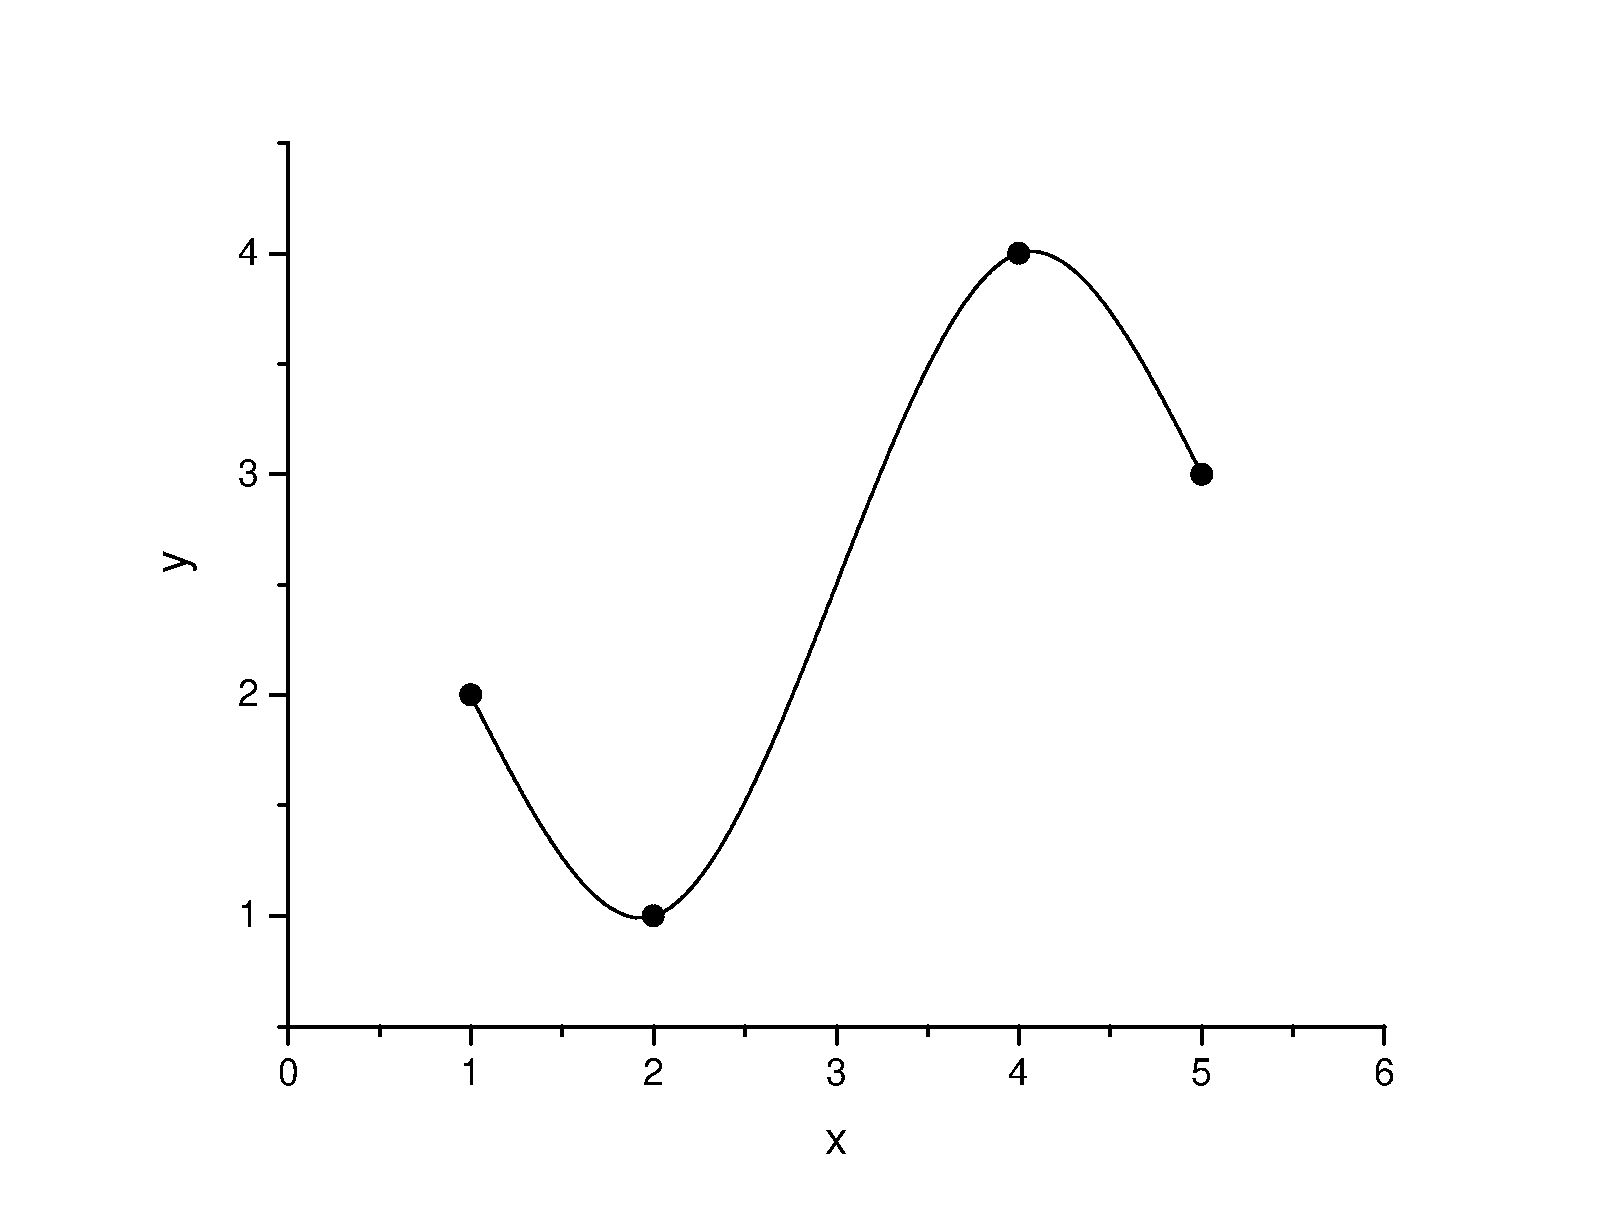
\includegraphics[width=5.5cm]{ch4/spline2}
    }
    \caption{\label{fig:spline}经过4点的线性样条插值与三次样条插值对比}
\end{figure}

多项值插值与样条插值是插值最常用的两种算法\cite{Timothy2018,Carl2008}。多项式插值给出满足所有原始数据点的单一公式,由于此过程中仅涉及浮点数加法与乘法,可以很方便的在PC及嵌入式设备上实现,因而得到广泛应用。
而样条插值则使用多个公式来通过所有数据点,其中每个公式均为低阶多项式。三次样条插值是样条插值在工业领域应用最广泛的算法之一,可以得到光滑的拟合插值曲线。
具体而言,对原始数据点$(x_1,y_1),(x_1,y_1),\cdots,(x_n,y_n)$,三次样条的插值曲线$S(x)$在每两个数据分段区间$[x_i,x_{i+1}]$内均使用三阶多项式
\begin{equation}
    \label{equ:spline}
    S_{i}=y_{i}+b_{i}(x-x_{i})+c_{i}{(x-x_{i})}^2+d_{i}{(x-x_{i})}^3
\end{equation}
并保证每两个多项式在端点(即原始数据点)处不仅数值相等,相应的斜率与曲率均相等,即
\begin{equation}
    \label{equ:cubiccha}
    \left \{
    \begin{aligned}
        S_{i}(x_{i})&=y_i,&\text{i=1,$\cdots$,n-1}\\
        S_{i}(x_{i+1})&=y_{i+1},&\text{i=1,$\cdots$,n-1}\\
        S_{i}^{'}(x_{i-1})&=S_{i}^{'}(x_{i}),&\text{i=2,$\cdots$,n-1} \\
        S_{i}^{''}(x_{i-1})&=S_{i}^{''}(x_{i}),&\text{i=2,$\cdots$,n-1}
    \end{aligned}
    \right.
\end{equation}
使用微积分的定义,将\autoref{equ:spline}代入\autoref{equ:cubiccha}化简整理后,可以得到包含$3n-5$个独立方程的方程组。另一方面,由于每个局部$S_i$中有三个未知参数,一共有$3n-3$个待解参数,则此时由线性代数相关知识可知,该方程组有无穷多组解。
即此时可以构造处无穷多条通过所有数据点$(x_i,y_i)$的样条曲线。因此,需要添加额外的方程对样条曲线进行约束,一般的约束条件都是对样条左右端点处进行限定 ,常见的附加边界条件如\autoref{tab:splinekind}所示\cite{Timothy2018}。
\begin{table}[htbp]
    \centering
    \caption{\label{tab:splinekind}几种常见的三次样条端点条件}
    \begin{tabularx}{\linewidth}{X<{\centering}X<{\centering}}
        \toprule 
        \textbf{样条种类}&\textbf{端点条件}\\
        \midrule 
        自然三次样条&
        $
            S_{1}^{''}(x_{1})=0,
            S_{n-1}^{''}(x_{n})=0
        $
        \\
        曲率调整三次样条&
        $\left \{
        \begin{aligned}
            &S_{1}^{''}(x_{1})=v_1,&v_{1}\neq0\\
            &S_{n-1}^{''}(x_{n})=v_n,&v_{n}\neq0
        \end{aligned}
        \right.
        $
        \\
        钳制三次样条&
        $\left \{
        \begin{aligned}
            &S_{1}^{'}(x_{1})=v_1,&v_{1}\neq0\\
            &S_{n-1}^{'}(x_{n})=v_n,&v_{n}\neq0
        \end{aligned}
        \right.
        $
        \\
        抛物线端点三次样条&
        $
            d_1=0,d_{n-1}=0
        $
        \\
        非纽结三次样条&
        $
            d_1=d_2, d_{n-2}=d_{n-1}
        $
        \\
        \bottomrule
    \end{tabularx}
\end{table}

在补充\autoref{tab:splinekind}中的两个端点条件公式后,即可完成上述方程组求解,从而确定唯一的三次样条插值曲线。本研究中三次样条算法基于自然边界条件对PPG信号进行均匀插值\cite{ttk2021},使信号采样率被提高至2000$Hz$。
\subsection{数据标准化}
在上述各项预处理过程完成后,此时得到的PPG数据在波形幅值上仍然有很大的个体差异,即使对同一被试对象,其波形在幅值上也会有一定的波动。为消除个体差异对特定波形特征计算的影响,需要对脉搏波信号进行归一化处理。
时间标准化与幅值标准化是PPG标准化两类常见的方式\cite{mmt}。时间标准化的基本原理是将PPG信号进行分组并计算每组信号的平均心动周期,随后对每组内的PPG信号进行时间尺度上的缩放,使最终的总平均心动周期保持一致。
由于不同个体的时间尺度上的缩放比例不一致,很容易导致PPG信号波形发生畸变失真,严重影响后续特征计算。故本研究采取了幅值标准化的处理方式对PPG信号进行处理。
由第二章PPG信号光学采集的基本原理可知,PPG信号的波形幅值对不同个体而言并无实际的生理意义,这保证了对PPG信号幅值标准化的合理性。与去除基线漂移过程类似,对待处理的特定PPG波形内所有采样点进行一次线性变换即可完成处理。
为使后续特征计算各项数值不会出现大量的小数,本研究没有采用最常见的归一化处理,而是将单个波形内所有数据点按同一尺度缩放映射到$[0,1000]$区间内。这一处理过程如所示。

另一方面,对于同一被试的不同PPG波形而言,其幅值的相对高低变化可能蕴含了一定的生理信息。因此,本小节的处理过程并没有与前文中的同为线性变换的去除基线漂移过程精简合并。在标准化过程中,所有波形的标准化系数即缩放比例也同时保存记录下来。
\section{脉搏波时域特征研究现状}
1. AIx

2. PWV

3. PSI

4. ADR

5. PTT

\section{时域特征参数设计与特征集构建}
\subsection{角度、幅值、长度等}
\section{小结}